\documentclass[12pt]{article}
        \usepackage{graphicx,type1cm,eso-pic,color}
        \usepackage{hyperref}
        \usepackage[left=3.0cm,right=3.0cm,top=2cm,bottom=2cm,headheight=13.6pt]{geometry}
        \usepackage{subfigure}

\makeatother


\title{Manual for CLAS12 FT-Hodo v1.0}

\author{FT-Cal On-Call Cell Phone: 757-810-1489 \\ 
Authors: \\
General contact: Gary \textsc{Smith} (\texttt{gsmith23@ph.ed.ac.uk})\\ 
General contact: Dan \textsc{Watts} (\texttt{dwatts1@ph.ed.ac.uk})\\ 
}

\date{\today} %01/07/2014

\begin{document}
\maketitle{}

\tableofcontents

\newpage
   \section{General description of the FT-Hodo}
The primary task of the Forward Tagger Hodoscope (FT-Hodo) is to separate electron and photon events in the calorimeter. These events cannot be distinguished using information from the FT-Cal alone due to the similarity of their electromagnetic shower shapes. Electrons are identified by observing the presence of a hit in the FT-Hodo array, which is correlated in both position and time with a cluster observed in the calorimeter. 

The FT-Hodo provides a highly efficient charged particle signal with a spatial and timing resolution similar to that of the calorimeter. In addition, to minimise possible misidentification of photons the detector is designed to suppress the contribution of false events arising from photon conversion in the FT-Hodo detectors and contributions from ``splashback" of the electromagnetic shower created by events depositing energy in the FT-Cal. To do this, a 2 layer design was implemented. The timing resolution of the FT-Hodo is comparable with FT-Cal so as not to compromise the achievable coincidence timing resolution (better than 1~ns).  The hodoscope is positioned upstream of the FT-Cal, fitting into a circular disk of diameter 330~mm and depth of 42~mm.

The hodoscope comprises a segmented array of plastic scintillator tiles (Eljen-204), embedded with a wavelength shifting (WLS) fibres, and is read out by 3x3~mm$^2$ silicon photomultipliers (SiPM) via optical fibres. The plastic scintillators provide fast timing and sufficient resistance to radiation damage for use in the high rate environments of the forward tagger. The scintillation light from the detector elements is transferred away from the hodoscope using embedded WLS fibres, which are fusion spliced to 5m-long optical fibres. The WLS fibres absorb the UV light produced in the plastic scintillator and emit at a larger wavelength (green), which matches well with the optimal quantum efficiency of typical SiPMs. The splicing induces a photon loss of less that 2\% whereas the use of optical fibre allows the captured light to be transported with a light loss less that $\sim40\%$ over the 5 meter path to the SiPM. 
\begin{figure}[h!]
   \begin{center}
   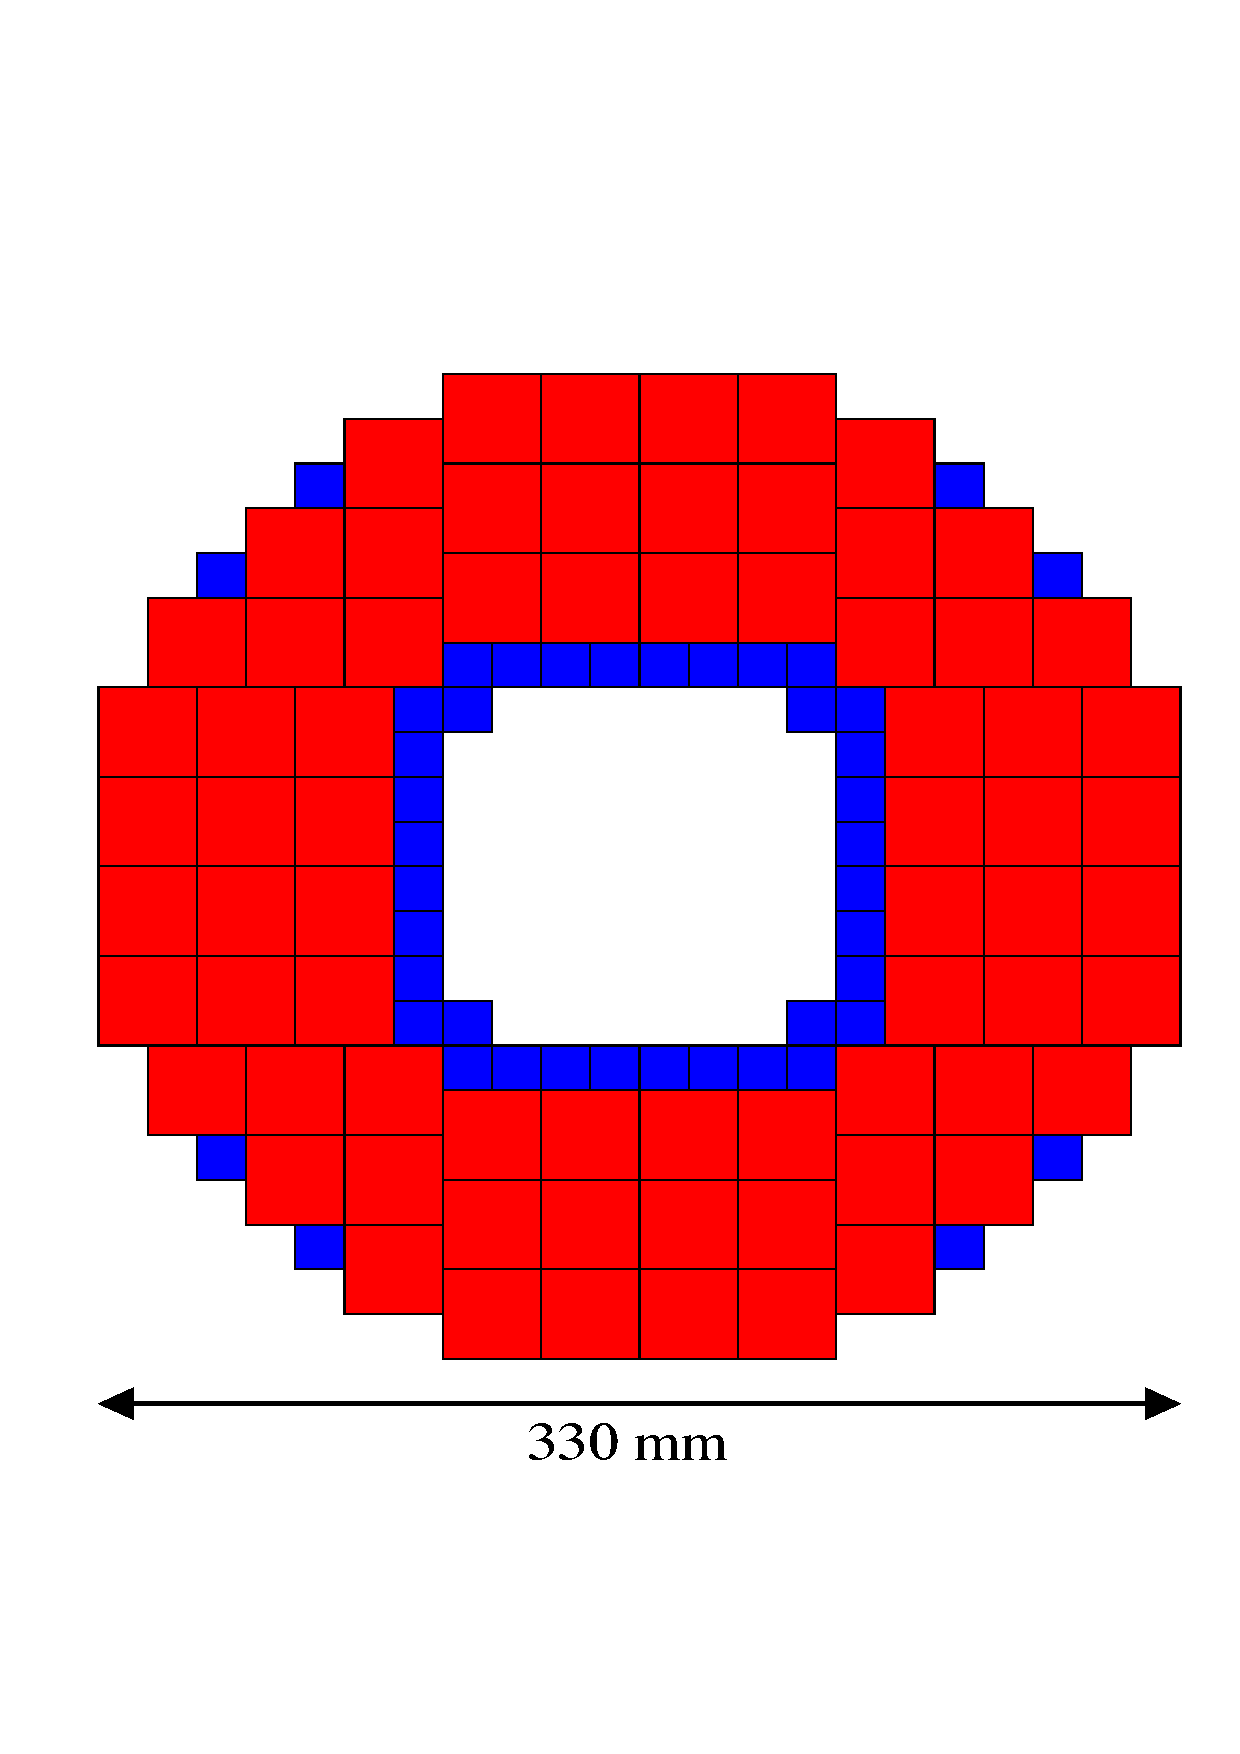
\includegraphics[width=3.0in]{HodoscopeArrayElement.pdf} 
   \caption{ Layout of plastic scintillator detectors in the Forward Tagger hodoscope. Blue squares represent 15 x 15 mm pixels and red 30 x 30 mm. }      \label{Fig:HodoscopeArrayElement}
   \end{center}
\end{figure}

The hodoscope array is made of two scintillator-tile sizes, 15 x 15 mm -- P15, and 30 x 20 mm -- P30, which cover a single and an array of four calorimeter crystals respectively. The arrangement of these detector elements that makes up a layer of the hodoscope is shown in Fig.~\ref{Fig:HodoscopeArrayElement}. The hodoscope comprises of 2 detector layers, each having 44 P15 and 72 P30 pixels. One layer is made from 7~mm-thick plastic scintillator tiles with the second utilising 15~mm-thick tiles. The two layer resolution is the preferred option for the hodoscope, sine the front thin layer is employed to reduce photon conversion in the hodoscope, while the thicker back layer provides the signal with the most accurate timing information for the event. 


\section{LED flasher}

\subsection{Overview}

The purpose of the LED flasher is to monitor changes in the transmission of the Hodoscope fibres. The principle of its operation is that pulsed light from an LED of a similar wavelength to that produced in the hodoscope scintillators is conveyed inside the hodoscope, to the enclosed area behind the scintillator tiles, and used to illuminate the part of the wavelength-shifting fibres which is outside the tiles. These absorb some of that light in the same way as they do the scintillation light, re-emit it inside the fibre at a longer wavelength and the light pulse is then transported down the optical fibre to the SiPM sensor at its end. Any changes in the behaviour of the wavelength-shifting fibres or the transmission of the optical fibres, for example due to radiation damage, will affect the read-out signal. A fraction of the emitted light from the LED will be measured directly with a SiPM to provide a calibration reference for each pulse. In order to decouple any possible effects due to the degradation of the flasher fibres, two single fibres of the same material and twice the length are passed from the LED through the hodoscope enclosure, one in each layer, and out to two SiPM sensors. The flasher can be pulsed at any time in a dedicated run. In this way any changes in the flasher signals read-out by the hodoscope fibres can be monitored over time, calibrated to the size and width of the emitted LED pulse and corrected for any degradation due to the flasher fibres themselves.  

\subsection{The flasher hardware}

The hardware comprises an LED light source with peak emission at 420 nm (M420F2, Thorlabs), the light from which is transported along a short optical fibre to a custom-made splitter, whence it travels along optical fibres into the hodoscope enclosure. 

The splitter has been custom-made at Glasgow University and consists of a small, light-tight plastic unit which houses a glass diffusing disk positioned in front of the LED fibre, a short cylindrical light-guide and a ``top hat'' fixture at the end containing the optical fibres. Eight output flasher fibres are fixed inside the rim of the ``top hat'' in a circle, their open ends meeting the light-guide. Additionally, a calibration fibre and two flasher-monitoring fibres are positioned in the centre of the ``top hat'', within the protruding cylinder inside which a number of transmission filters reduce the light intensity down to a level that is not damaging to the SiPM sensor. The calibration fibre is connected directly to a SiPM and its signal is used to calibrate the LED pulse read out from the hodoscope channels. The two flasher-monitoring fibres are passed through the hodoscope enclosure, one through each layer, and connected directly to SiPMs. They are made from the same material as the flasher fibres and any changes in the signals sent through them are used to quantify degradation effects of the flasher fibres.     

The tips of the flasher fibres have been machined to emit diffuse light homogeneously along their length, illuminating the hodoscope enclosure inside which they are positioned. The configuration can be seen in Fig. \ref{glow_stick_in_situ}, with 6 cm long tips epoxied to the hodoscope lid tangentially in the centre of the hodoscope fibres closer to the neck of the hodoscope and 9 cm long tips epoxied in the equivalent positions further from the neck. Thus, in each of the two layers of the hodoscope, four illuminating tip fibres are fixed to the lid of the hodoscope tracing out a rough circle in the middle of its active part. The illuminating-tip fibres were 6m long, produced by Medlight (cylindrical light diffusers, model RD) with a $500 \mu m$ diameter plastic core, clad in transparent PVC plastic ($1/1.8$ mm inner/outer diameter) sealed at the illuminating end. The part of the fibre which is outside the hodoscope enclosure was additionally sheathed in black plastic tubing to provide a light-seal. The two flasher-monitoring fibres, 12 m long, were made of the same material but without an illuminating end. These were stretched through the two layers of the hodoscope and epoxied to the lid alongside the illuminating tips.

\newpage
\part{Shift Takers Instructions}

All FT-Hodo controls are accessible through EPICS, from the main HPS\_EPICS window (figure~\ref{EPICSmain}).  If not already running, it can be opened by executing
the command \begin{center}\texttt{hps\_epics}\end{center} in a terminal on any of
the \texttt{clonpc\#\#} workstations in the Hall-B counting house.

{\em   All shift workers should be using user \texttt{hpsrun} for all instructions in this document.}

The primary FT-Hodo screen is shown in figure~\ref{fig:ecal_all} and opened via t
\vspace*{\stretch{1}}      
%\%\%\%\%\%\%\%\%\%\%\%\%\%\%\%\%\%\%\%\%\%\%\%\%\%\%\%\
\begin{figure}[h!]
\center
%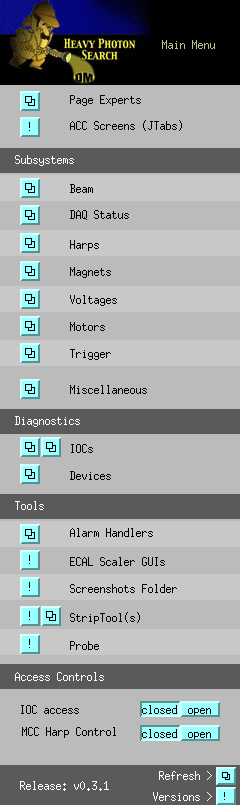
\includegraphics[width=0.38\textwidth]{pics/hps_epics_2014_12_15.png}
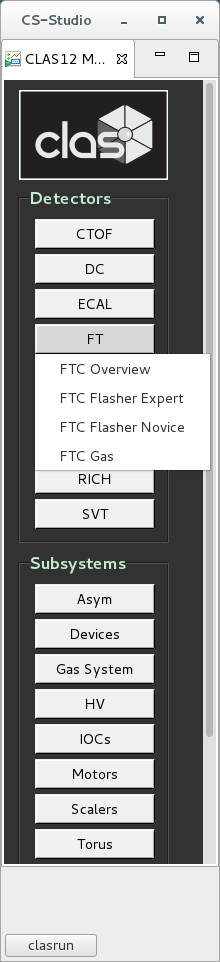
\includegraphics[width=0.20\textwidth]{Images/clascss_main_menu_FT_selection.png}
\caption{ \label{EPICSmain} View of the Hall-B EPICS main window.Menu shown gives access to the HV, LV, Temperature sensors, Chiller, Gas system, and LED flasher.}
\end{figure}
\section{Primary FT-Hodo EPICS Screen}

\newpage

\section{Low Voltage}
{\em The low voltage power supply must be on before HV is turned on, and changing its settings requires contact with an FT-Hodo-expert.}
      
LV should be monitored using its webcam and its portion of the main ECAL EPICS screen (both shown in figure~\ref{LVCam}). Call the FT-Hodo expert if this appears not to be ON or shows an abnormal current for either of its two channels.  {\em Normal current is between 4.0 and 4.2 A for both channels}.  This webcam is accessible via the url \texttt{cctv11.jlab.org} in a web browser and the ``Monitoring'' tab on the main {\bf HPS Run Wiki}.

%\%\%\%\%\%\%\%\%\%\%\%\%\%\%\%\%\%\%\%\%\%\%\%\%\%\%\%\
\begin{figure}[htbp]
\center

%\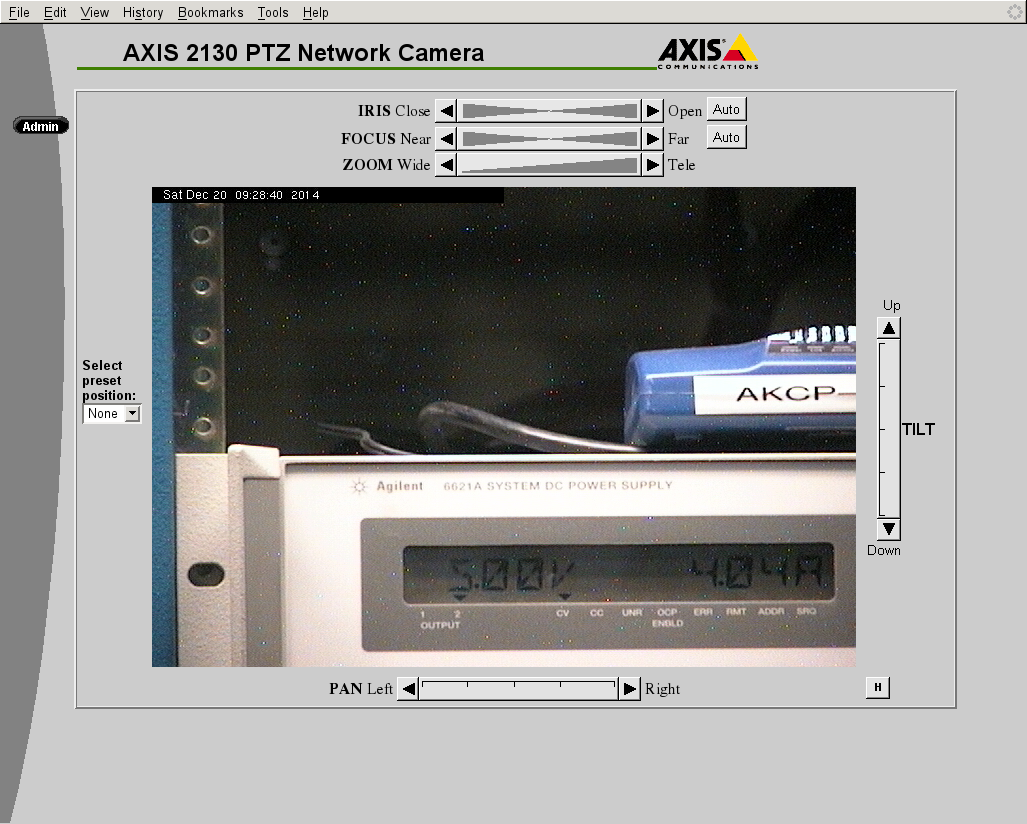
\includegraphics[width=0.49\textwidth,height=5.5cm]{pics/LVCam_2014_12_20.png}
%\%\%\%\%\%\%\%\%\%\%\%\%\%\%\%\%\%\%\%\%\%\%\%\%\%\%\%\
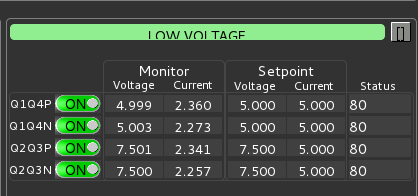
\includegraphics[width=0.39\textwidth,height=5.5cm]{Images/LV.png}
\caption{ LV controls for the FTHodo.LV STRIP CHARTS TO BE IMPLEMENTED SOON}
\end{figure}
%\%\%\%\%\%\%\%\%\%\%\%\%\%\%\%\%\%\%\%\%\%\%\%\%\%\%\%\

\section{High Voltage}
      \subsection{Turning ON/OFF High Voltages}

      The high voltage supply of the FT-Hodo is controlled and monitored using the main FT-Hodo
EPICS window (Figure ~\ref{fig:ecal_all}).  It has buttons to ramp up and down the entire 
hodoscopes high voltages (labeled {\bf ALL ON} and {\bf ALL OFF}), open windows for
individual channel control (figure~\ref{HVControl}), and open more detailed expert views 
(e.g. figure ~\ref{HV}).

   \subsection{HV Current Monitoring}
   Individual channels' currents can be monitoring in figure~\ref{HVControl}, and strip charts should be open for long term monitoring.  The strip charts are accessible from the main FT-Hodo screen (figure ~\ref{fig:ecal_all}) under the HV sections' {\bf Monitors} button (and also from the HPS\_EPICS screen (figure~\ref{EPICSmain}) via the {\bf Strip-Tool} button).  An example is shown in figure~\ref{fig:hvcurrentstrips}.  Jumps or drifts in current of more than 1 A should be noted in the logbook.
   
   
%\%\%\%\%\%\%\%\%\%\%\%\%\%\%\%\%\%\%\%\%\%\%\%\%\%\%\%\
%   \begin{figure}[htbp]\centering
%       \includegraphics[width=16cm]{pics/**********.png}
%       \caption{HV Current strip charts. TO BE ADDED.\label{fig:hvcurrentstrips}}
%   \end{figure}
%\%\%\%\%\%\%\%\%\%\%\%\%\%\%\%\%\%\%\%\%\%\%\%\%\%\%\%\

   \subsection{Responding to HV trips}

   HV problems, in particular trips, are indicated by a red group in the main FT-Hodo EPICS GUI (figure~\ref{fig:ecal_all}).  HV trips will also be announced by the alarm handler.  During normal operations with HV ON, there should be no red groups in Figure \ref{fig:ecal_all} and no ECAL HV alarms.  In case of an HV trip, or a red region in Figure \ref{fig:ecal_all}:
\begin{itemize}
    \item Try to reenable the tripped HV group by turning it back on in the EPICS HV control screen (figure~\ref{HVControl}) accessed via the {\bf Controls} button in the main FT-Hodo EPICS screen (Figure \ref{fig:ecal_all}).  (An easier alternative is just pressing the {\bf ALL ON}
button in the main FT-Hodo EPICS screen.)
    \item Record the trip in the log book with precise indication of the group and run
        number concerned. 
\end{itemize}
Contact the ECAL expert on-call in case of uncertainty.
      
      {\em Note, the HV can take up to 3 minutes to turn back on so you should end the current run and begin a new one when the high voltage is back on. If you cannot get a HV group to work contact the FT-Hodo expert on call.}

      {\bf If you encounter more than two HV trips during your shift for the same group, you should notify the FT-Hodo Expert.}


%\%\%\%\%\%\%\%\%\%\%\%\%\%\%\%\%\%\%\%\%\%\%\%\%\%\%\%\
\begin{figure}[htbp]
\center
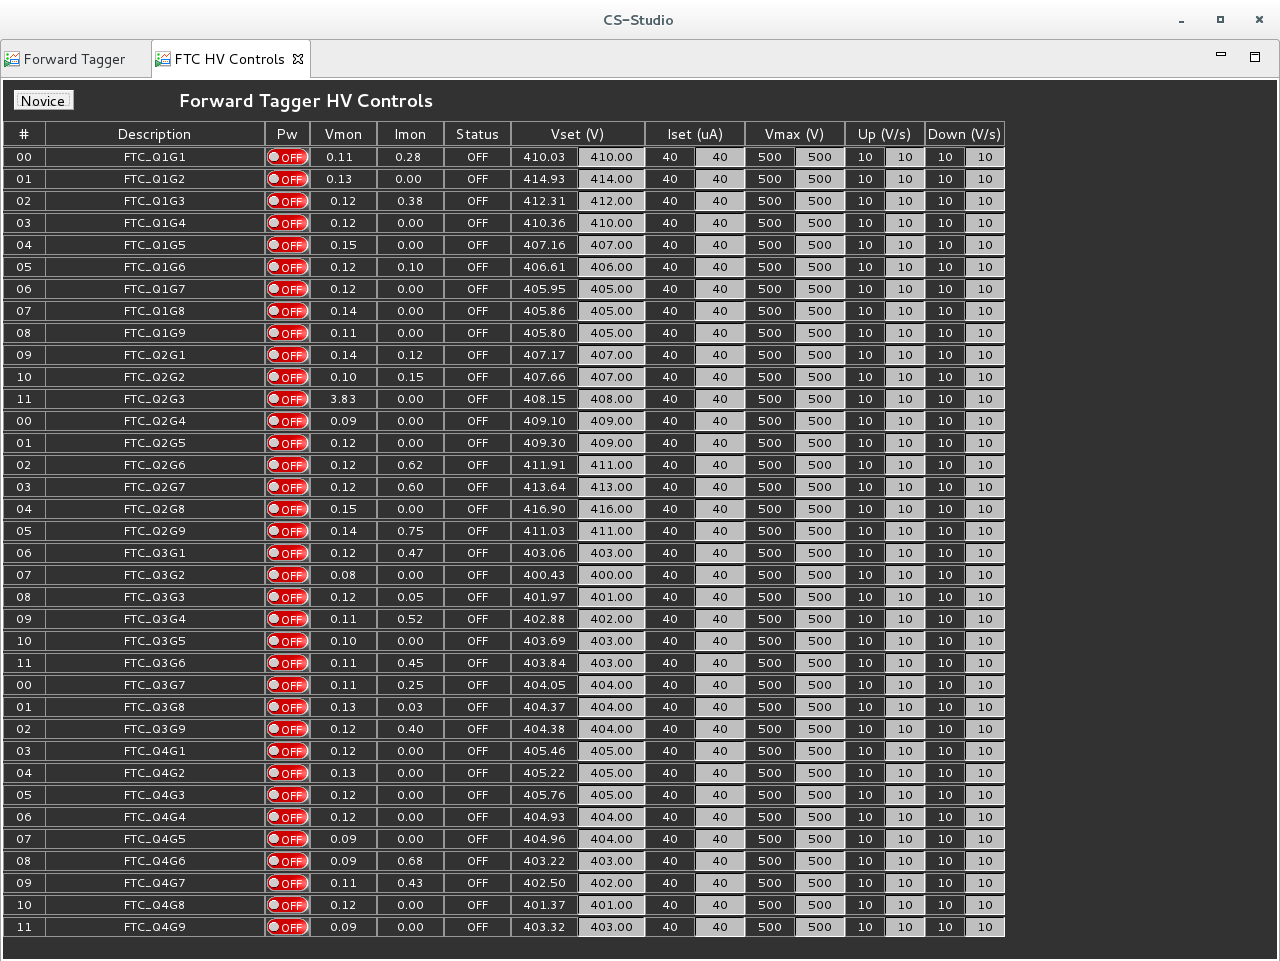
\includegraphics[width=0.85\textwidth]{Images/FTC_HV_controls_expert.png}
\caption{ \label{HVControl} Cropped view of the EPICS FT-Hodo HV control window for individual channels.}
\end{figure}
%\%\%\%\%\%\%\%\%\%\%\%\%\%\%\%\%\%\%\%\%\%\%\%\%\%\%\%\



\clearpage

\newpage
      \section{Scalers}

      Rates seen by the FT-Cal are available in the ROOT-based GUI shown in Figure \ref{Scalers}, which represent the rates as seen by the FADC electronics.  This display is accessible via the main HPS\_EPICS window under the {\bf ECAL Scaler GUIs} button, and also by running the command \texttt{hps\_ecal\_scalers} in a terminal.  {\em As of 2016, the discriminators are disconnected and only the FADC rates are accessible.}
      
      One can also see clustering scalers from the DAQ ``diaggui'' screen (figure~\ref{DAQscalers}), accessible also by the {\bf ECAL Scaler GUIs} button or by executing \texttt{diaggui.sh} in a terminal.  This GUI indicates the rates of clusters reconstructed by the trigger electronics. 
      
      These numbers should all remain constant within $^\sim10\%$ during stable beam operation. A strong increase is the indication of bad beam conditions or the presence of a new source of noise in the FT-Cal system.  If the latter case, please contact FT-Cal expert on call.
%\%\%\%\%\%\%\%\%\%\%\%\%\%\%\%\%\%\%\%\%\%\%\%\%\%\%\%\      
\begin{figure}[htbp]
\center
%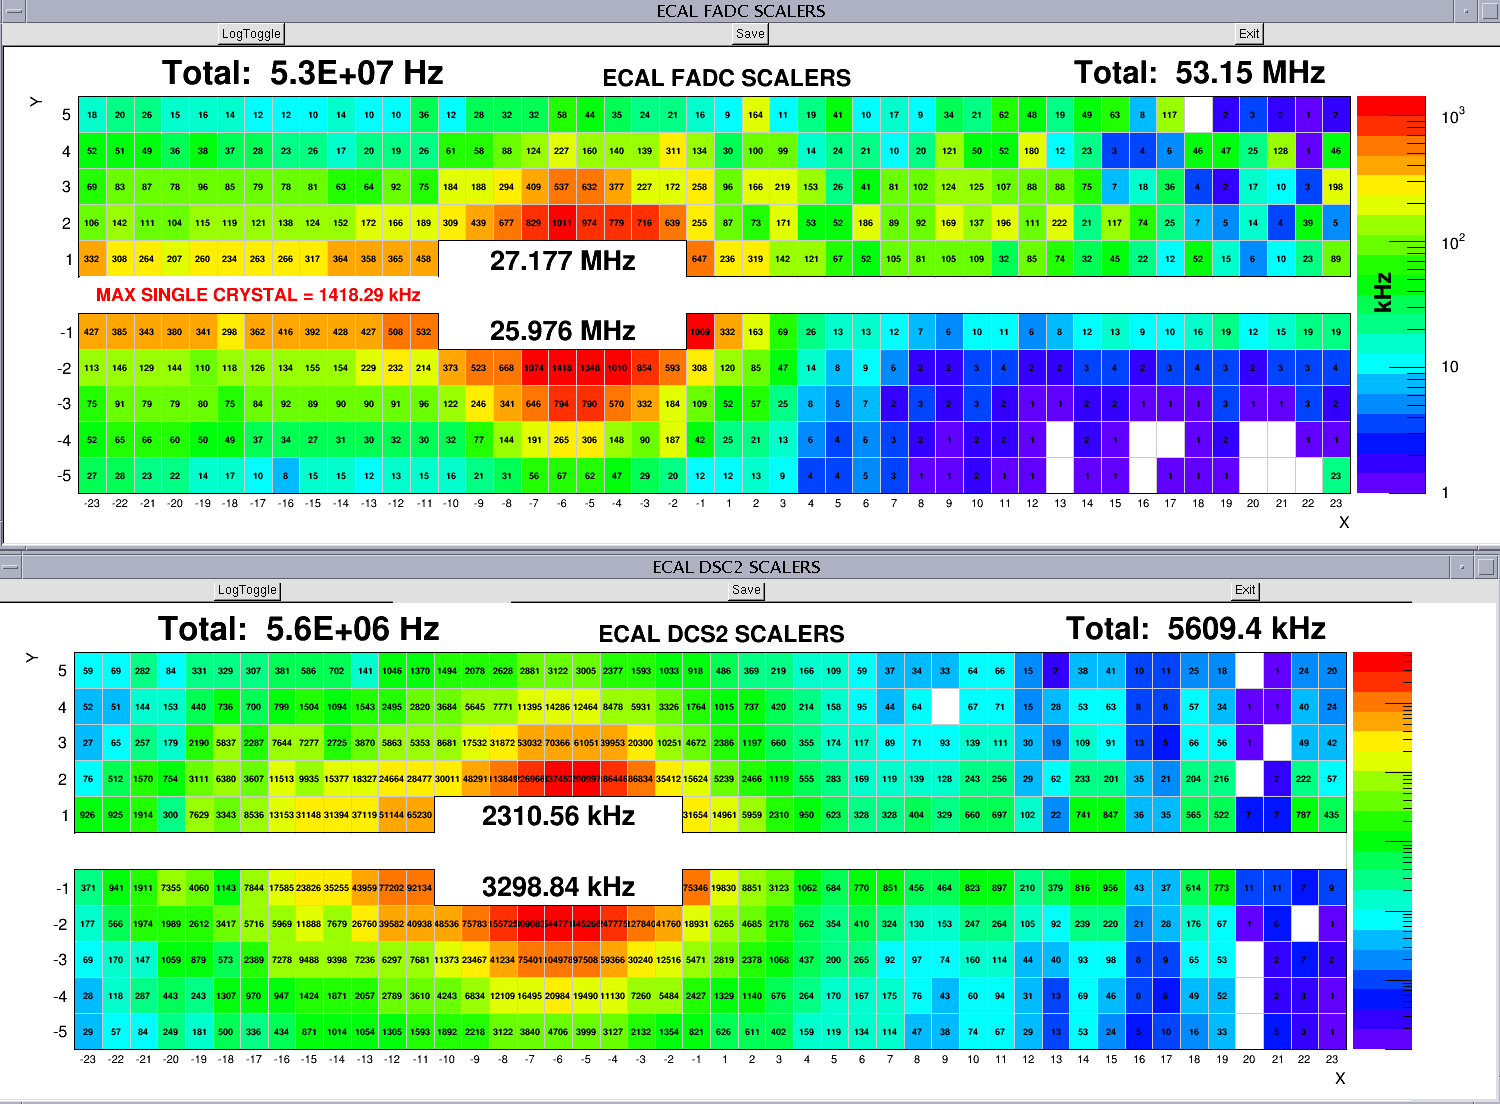
\includegraphics[width=0.75\textwidth]{pics/ECAL_FADC_SCALER_2014_12_20.png}
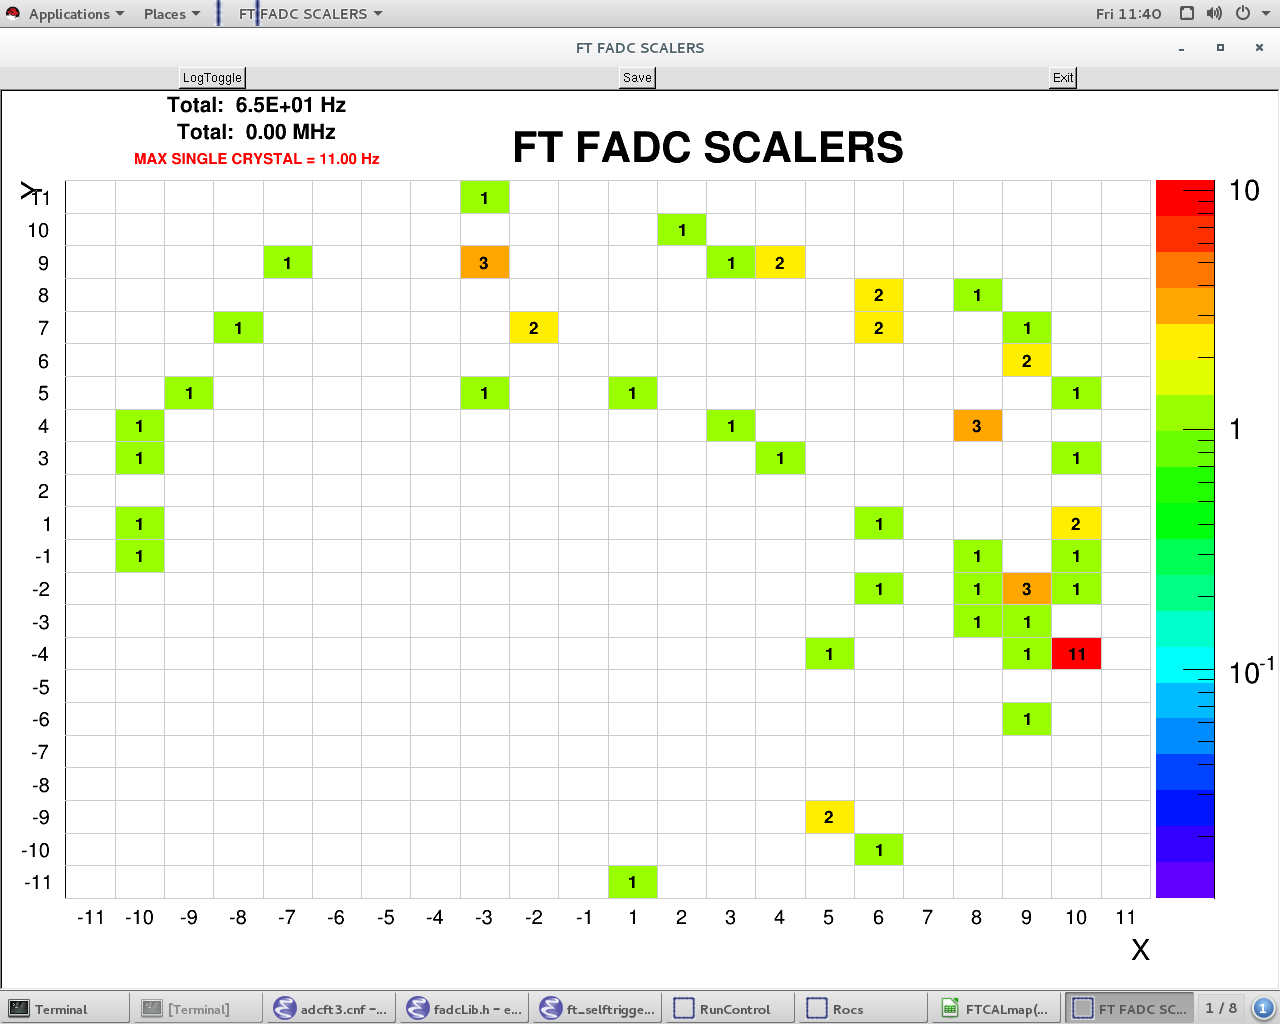
\includegraphics[width=0.9\textwidth]{Images/Scalers.png}
\caption{ \label{Scalers} View of the EPICS FADC scalers window.}
\end{figure}
%\%\%\%\%\%\%\%\%\%\%\%\%\%\%\%\%\%\%\%\%\%\%\%\%\%\%\%\
%\%\%\%\%\%\%\%\%\%\%\%\%\%\%\%\%\%\%\%\%\%\%\%\%\%\%\%\
%\\begin{figure}[htbp]
%\\center
%\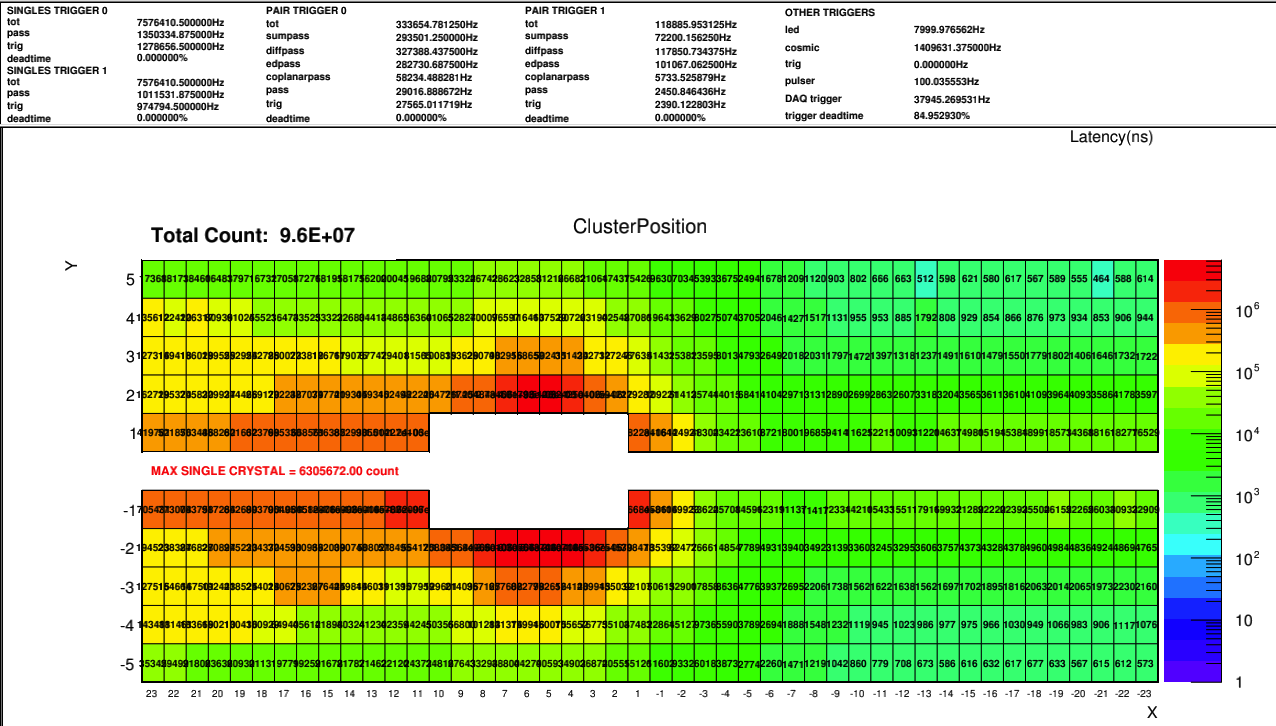
\includegraphics[width=0.9\textwidth]{pics/ecal-cluster-12-20-14.png}
%\\caption{ \label{DAQscalers} View of the DAQ scaler window.}
%\\end{figure}
%\%\%\%\%\%\%\%\%\%\%\%\%\%\%\%\%\%\%\%\%\%\%\%\%\%\%\%\

\newpage
  \section{Strip Charts}
      The most import quantities to monitor with strip charts are temperature and HV current.  There are two programs to view strip charts of FT-Cal EPICS variables.  The older StripTool shown in figure~\ref{temp2} can be started from the HPS\_EPICS gui.  The newer MyaViewer (which adds the ability to retrieve archive information) can be run by executing the following scripts in a terminal:
      
      \begin{itemize}
          \item \texttt{mya\_ecal\_all.sh}
          \item \texttt{mya\_ecal\_temp.sh}
          \item \texttt{mya\_ecal\_curr.sh}
          \item \texttt{mya\_ecal\_voltage.sh}
      \end{itemize}



\section{Monitoring App}
The monitoring application is based on the common tools developed for CLAS12. It provides many plots to assess detector performance.  To start the monitoring app, in a terminal run:
\begin{center}\texttt{startHodoMonitoring}\end{center}
%Then click the ``connect'' button to connect to the ET ring.

 After a few minutes of beam, the tabs should be cycled through and their plots compared to the reference.  Once sufficient statistics are accumulated, the plots should be saved as a pdf and uploaded to the logbook.

The main window is split into two panels 1) the detector view, and 2) data view. The detector view shows the individual tiles in the two hodoscope layers and allows the selection of a specific detector element. It also indicates bad detector elements through colour-coding. The data view shows information collected using the selected detector element. 

%\section{Taking a Cosmic Calibration Run}
% \section{Taking a Pedestal Run}
%
% \subsection{With Beam}
%  \subsection{Without Beam}
%
%
%    \section{Taking a FEE Run for Gain Calibration}
%
%\newpage
%
\part{FT-Cal Experts Resources}

   \section{Location of FT-Hodo Elements}

   {\em{\bf REMINDER:} Since the FT-Hodo is within 3 feet of the beamline, it needs to be surveyed by RADCON before any work can be done on it.}
  {\footnotesize
\begin{itemize}

\item
The LED controllers are located at the top of the rack closest to the beamline in the Alcove.
\\item
The FADCs and patch panels occupy the rack furthest from the beamline in the Alcove.
\item
    The HV supply is on the Pie Tower in the rack closest to the beamline.  See figure~\ref{fig:HVPHOTO}.
\item
    The LV supply is on the Pie Tower at the top of the middle rack. See figure~\ref{fig:LVPHOTO}.
\end{itemize}
}%\%\%\%\%\%\%\%\%\%\%\%\%\%\%\%\%\%\%\%\%\%\%\%\%\%\%\%\
\begin{figure}[htbp]\centering
%    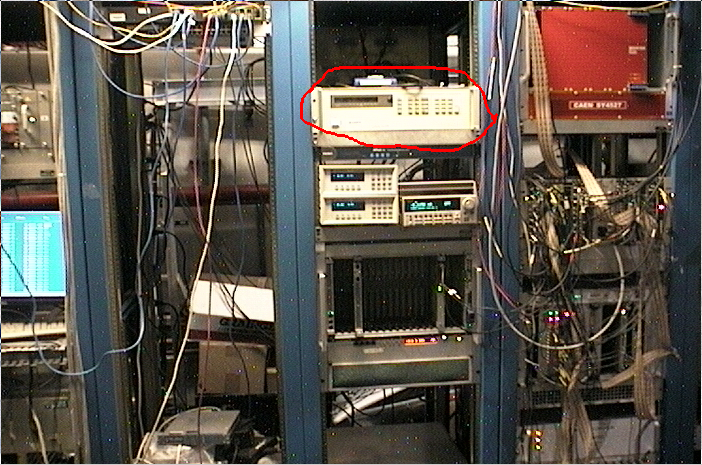
\includegraphics[width=7cm]{pics/ECALLVPHOTO2.png}
%    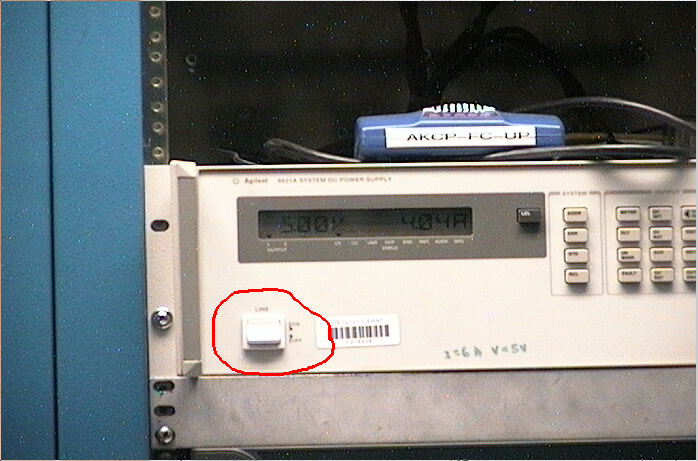
\includegraphics[width=7cm]{pics/ECALLVPHOTO.png}
    
\includegraphics[width=7cm]{Images/image.png}
    \caption{Location of Agilent LV power supply near the top of the middle rack in the pie tower.  Power switch is circled in red.\label{fig:LVPHOTO}}
\end{figure}
\begin{figure}[htbp]\centering
    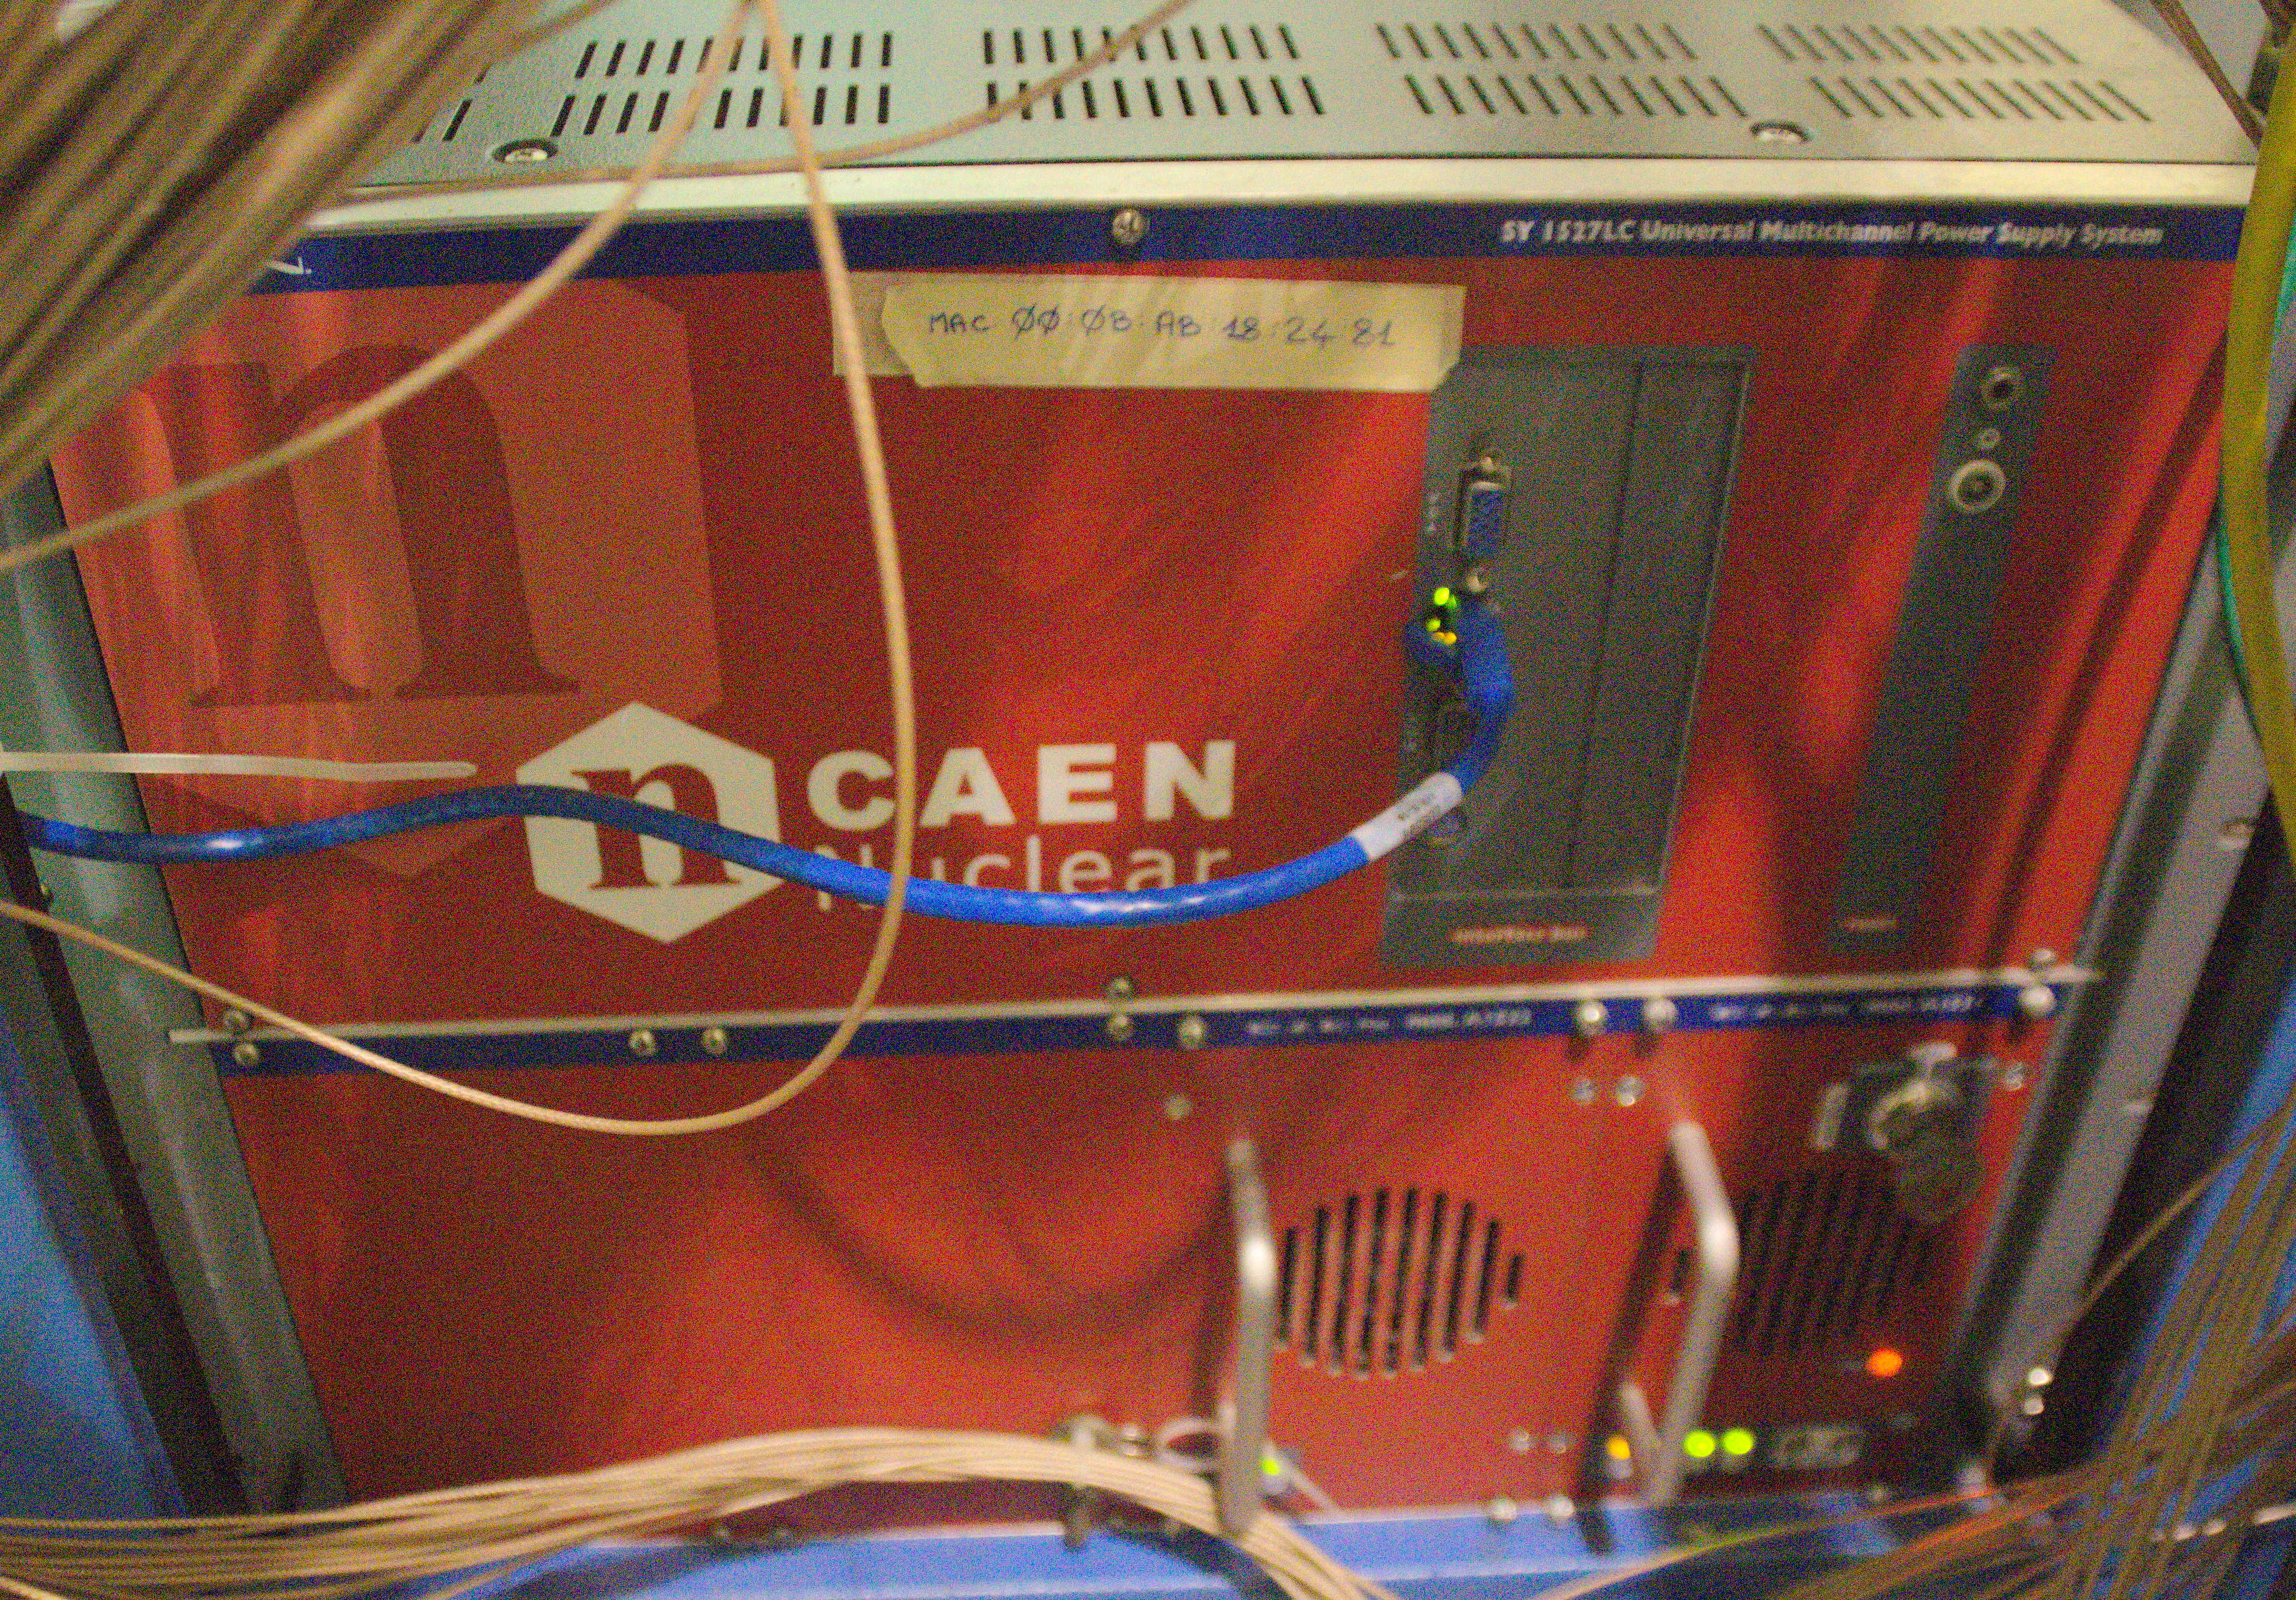
\includegraphics[width=9cm]{Images/CAEN.jpg}
    \caption{Location of the CAEN  HV power supply ****LOCATION TBA***.  Key for on/off is in the lower right corner of the crate.}
\end{figure}

\newpage
   \section{LV Supply}
 The low voltage power supply is an Agilent 6621.  It should be set with both channels at $+5$V with their current limits at 6 A, while external wiring inverts one channel to create a bipolar $\pm5$V supply. 

      The low voltage supply might have difficulties to get to full voltage because of high current. If that was the case check, with all power supplies off, that all connection are goods. Then contact run coordinator to see if LV power supply addition is possible. 

\subsection{Changing LV Settings}
The LV supply can be controlled via its EPICS expert screen (figure~\ref{lvexpert}), accessible from the grey button in the top right of the LV section of the main Hodo EPICS screen (figure~\ref{fig:ecal_all}). In general the only necessary changes are powering on/off, while voltage and current setpoints are never changed from 5V/6A.


{\em Note, as a safeguard, if one currently tries to use EPICS to set the voltage greater than 5 V or the current greater than 6 A, the request will be ignored by the IOC.}  Overriding these limits can currently only be done either via local control (Section \ref{sec:lvlocalops}), or by setting new values for the limits via \texttt{caput}.  The corresponding PVs are:
{\footnotesize
\begin{itemize}
    \item\texttt{HPSECALLV:i1set:DRVH}
    \item\texttt{HPSECALLV:i2set:DRVH}
    \item\texttt{HPSECALLV:v1set:DRVH}
    \item\texttt{HPSECALLV:v2set:DRVH}
\end{itemize}
}

\subsubsection{Local Operation}\label{sec:lvlocalops}
The LV supply can also be controlled manually in the hall via buttons on its front panel.  However, when in remote mode (denoted by the ``RMT'' marker in its LCD display), local operations require pressing the ``LCL'' button first, then quickly pressing the desired operation button before remote mode is automatically reenabled by the IOC.  Completely disabling this ``feature'' requires stopping the IOC (see section~\ref{lviocstop}).

\subsection{Restarting the LV IOC}
   To restart the IOC:
   {\footnotesize
   \begin{enumerate}
       %\item \texttt{`ssh hpsrun@clonsl1'}
       \item \texttt{`softioc\_console iocA6621'} and type user's password if necessary.
       \item \texttt{`ctrl-x'} to restart the IOC
       \item \texttt{`ctrl-]'} to quit to telnet
       \item \texttt{`quit'} to exit telnet
   \end{enumerate}
   }
\noindent{\em Don't leave a terminal open connected to this telnet session.}

\subsection{Disabling the LV IOC}\label{lviocstop}
   To disable the IOC:
   {\footnotesize
   \begin{enumerate}
       %\item \texttt{`ssh hpsrun@clonsl1'}
       \item \texttt{`softioc\_console iocA6621'} and type user's password if necessary.
       \item \texttt{`ctrl-t'} to toggle auto-restart
       \item \texttt{`ctrl-x'} to kill the IOC
       \item \texttt{`ctrl-]'} to quit to telnet
       \item \texttt{`quit'} to exit telnet
   \end{enumerate}
   }
\noindent{\em Don't leave a terminal open connected to this telnet session.}

\newpage
   \section{High Voltage}
   \subsection{Restarting the HV IOC}
   Occaissonaly the soft IOC for the HV needs to be manually restarted.  Symptoms of this condition include errors messages from EPICS when trying to turn on/off voltages and white blocks in the main HV screen (figure~\ref{HV}).  
   
   To restart the IOC:
   {\footnotesize
   \begin{enumerate}
       %\item \texttt{`ssh hpsrun@clonsl1'}
       \item \texttt{`softioc\_console iocecalVoltages'} and type user's password if necessary.
       \item \texttt{`ctrl-x'} to restart the IOC
       \item \texttt{`ctrl-]'} to quit to telnet
       \item \texttt{`quit'} to exit telnet
   \end{enumerate}
   }
\noindent{\em Don't leave a terminal open connected to this telnet session.}

{\bf\em Note, this IOC always needs to be restarted if the HV CAEN mainframe is power cycled.}
   
   \subsection{Changing HV Settings}
      {\bf NOTE:} Changing voltage settings should be taken care of in coordination with the FT-Cal group (contact M.~Battaglieri). Current setting can be increased in case of need, please document this change in the log book and notify the FT-Cal expert on call.

 {\bf NOTE:} The FT-Cal HV groups were renumbered for EPICS, and the correspondence map (figure~\ref{ExpertMap}) is available in the expert FT-Cal HV monitoring window (Figure 
 \ref{HV}) via the ``Expert HV Map'' button.

%\%\%\%\%\%\%\%\%\%\%\%\%\%\%\%\%\%\%\%\%\%\%\%\%\%\%\%\
\begin{figure}[htbp]
\center
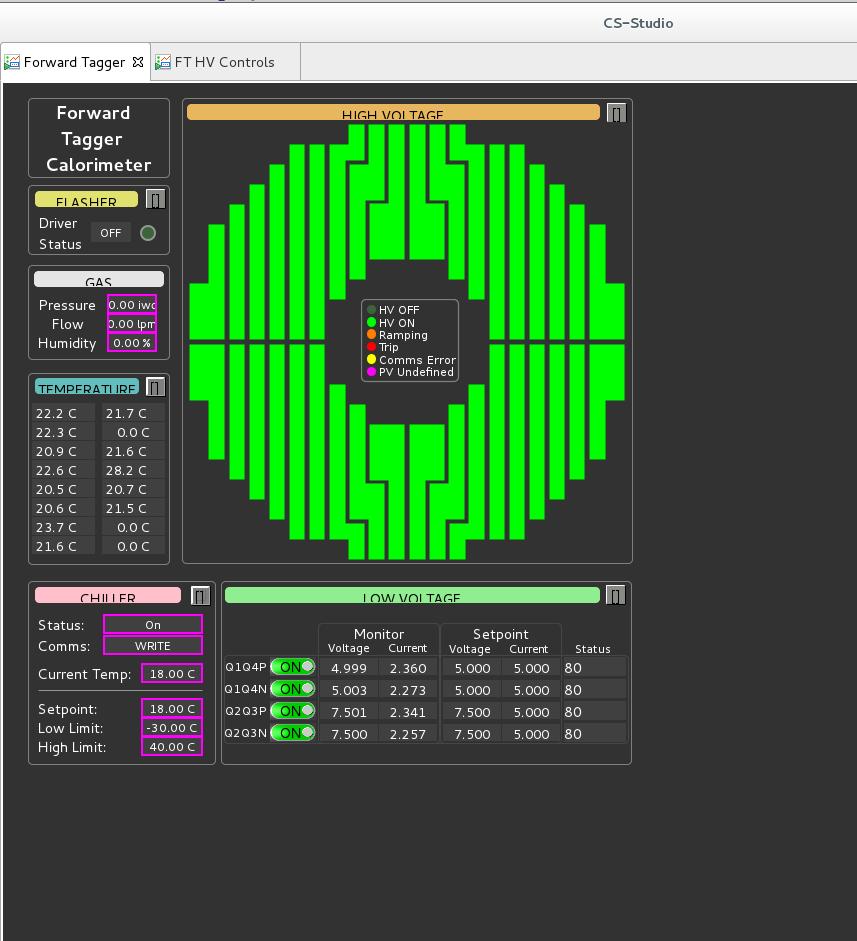
\includegraphics[width=0.95\textwidth]{Images/All_Working_HVs.png}
%\includegraphics[width=0.95\textwidth]{pics/ecalhv_2014_12_15_16:02:54.png}
\caption{ \label{HV} View of the EPICS FT-Cal HV expert monitoring window.}
\end{figure}

%\%\%\%\%\%\%\%\%\%\%\%\%\%\%\%\%\%\%\%\%\%\%\%\%\%\%\%\
\begin{figure}[htbp]
\center

\includegraphics[width=0.95\textwidth]{Images/image.png}
\caption{ \label{ExpertMap} HV channel map for reference.}
\end{figure}
%\%\%\%\%\%\%\%\%\%\%\%\%\%\%\%\%\%\%\%\%\%\%\%\%\%\%\%\

      If for some reason some channels were to drop in gain (or increase) or if the current drawn increases in a group, it might be necessary to change the HV settings in the expert FT-Cal EPICS control (Fig.~\ref{EHV}). A modification of the voltage will lead to a modification of the gain used by the trigger system, these values need to be updated at the same time!
    
      \subsubsection{HV Save/Restore}
      A system to save and restore the entire calorimeter's voltage settings is available via buttons in the ECAL HV expert window in Figure \ref{HV}.  If the voltage setpoints are changed, a backup should be made of the new settings.  This must be run as a user in group \texttt{clas-4};  user \texttt{hpsrun} does not have sufficient priveleges to save/restore voltage settings. 
      An example of the restore window is shown in figure~\ref{fig:hvrestore}, which is accessible from the HV expert screen shown in Figure~\ref{HV}.

%\%\%\%\%\%\%\%\%\%\%\%\%\%\%\%\%\%\%\%\%\%\%\%\%\%\%\%\
%\\begin{figure}[htbp] \centering
%\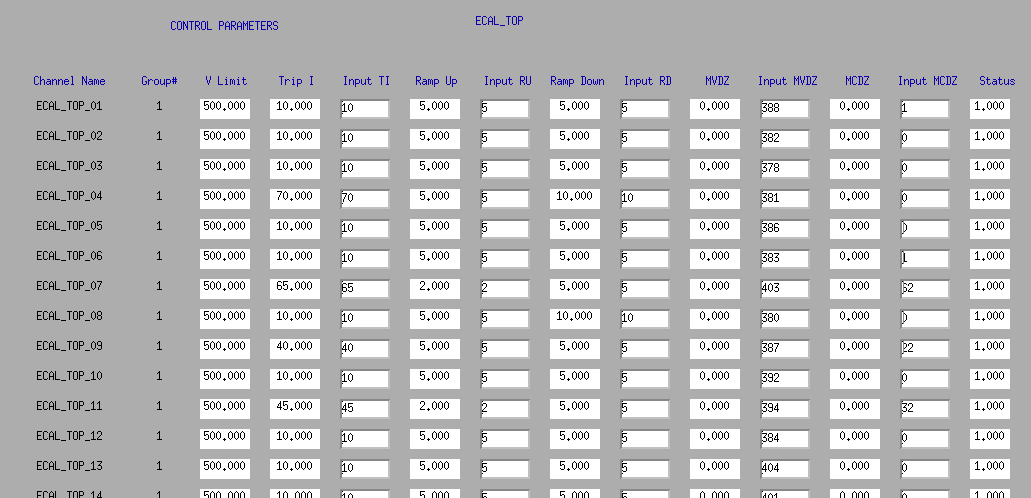
\includegraphics[width=0.85\textwidth]{pics/ecalhv_parameters_2014_12_15.png}
%\\caption{ \label{EHV} Cropped view of the EPICS HV expert control window. It is accessed from the parameters button in the FT-Cal HV control screen \ref{HVControl}}
%\\end{figure}
%\%\%\%\%\%\%\%\%\%\%\%\%\%\%\%\%\%\%\%\%\%\%\%\%\%\%\%\

   \subsection{Long Term HV monitoring}

   An hourly snapshot of HV currents is stored by a cron job (and in the EPICs and MYA databases).  Currently the easiest way to view it is as user \texttt{hpsrun} on \texttt{clonpcNN} by excuting the command:
   \begin{center}
   \texttt{\$HOME/.ecalhv/plotEcalHV.py}
   \end{center}
The product should be a plot like figure~\ref{HVhistory}.

\begin{figure}[htbp]\centering
    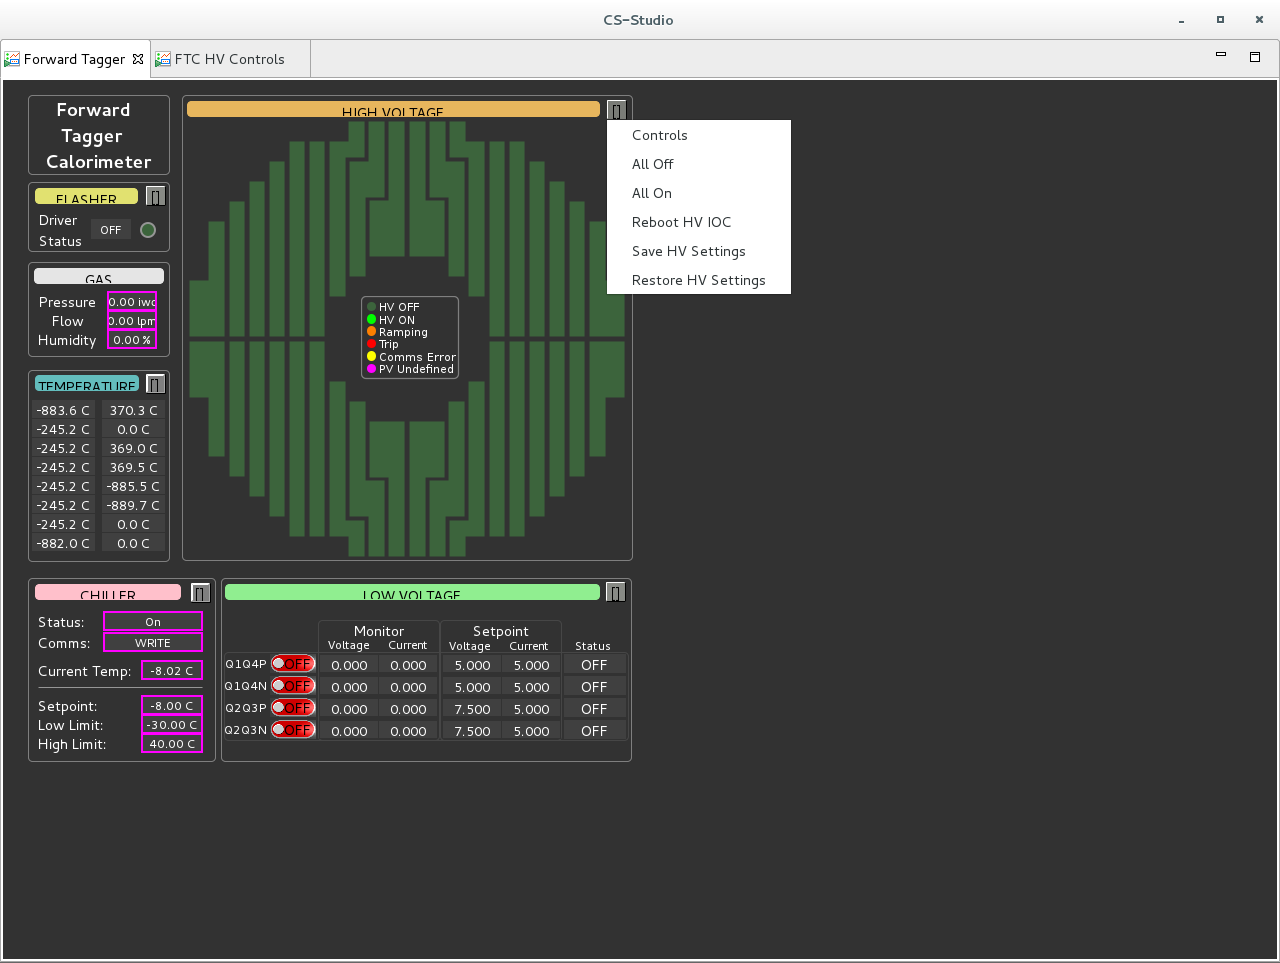
\includegraphics[width=8cm]{Images/FTC_HV_menu.png}
    \caption{HV menu within EPICS to save/restore HV settings.  \label{fig:hvrestore}}
\end{figure}

%\%\%\%\%\%\%\%\%\%\%\%\%\%\%\%\%\%\%\%\%\%\%\%\%\%\%\%\
%\\begin{figure}[htbp] \centering
%\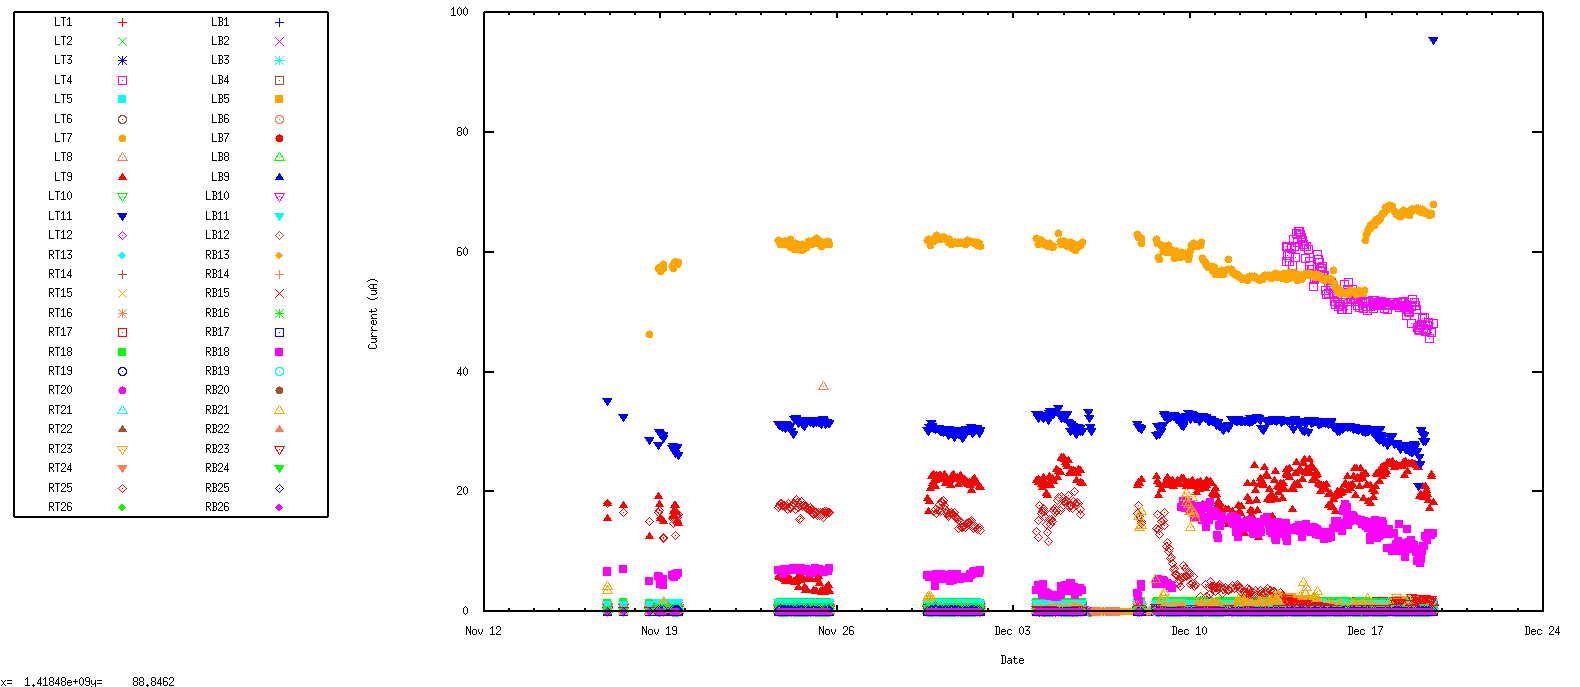
\includegraphics[width=0.95\textwidth]{pics/ECALHVCURRENTS_2014_12_20.png}
%\\caption{ \label{HVhistory} Expert HV current history.}
%\end{figure}
%\%\%\%\%\%\%\%\%\%\%\%\%\%\%\%\%\%\%\%\%\%\%\%\%\%\%\%\

\section{Channel Mapping GUI}
Channel mapping is available in a spreadsheet in the annex pdf on the HPS Run Wiki. It is also available in an interactive GUI (shown in Figure \ref{fig:kylesGui}) which can be run by executing \begin{center}\texttt{kylesGui.sh}\end{center} in a terminal.

The user can hover over a crystal with the mouse to see all its channel numberings in the table at the bottom of the window.  This includes x/y-indices, APD and LED channel numbers, FADC slot/channel, JOUT connector and channel, and HV group.  {\em Note that preamp numbers in this GUI are no longer copmletely correct after their partial replacements prior to the 2015 Engineering Run}.  

There is also a filtering option in the {\bf View} menu to highlight all channels corresponding to certain criteria.

%\%\%\%\%\%\%\%\%\%\%\%\%\%\%\%\%\%\%\%\%\%\%\%\%\%\%\%\
%\\begin{figure}[htbp]\centering
%\    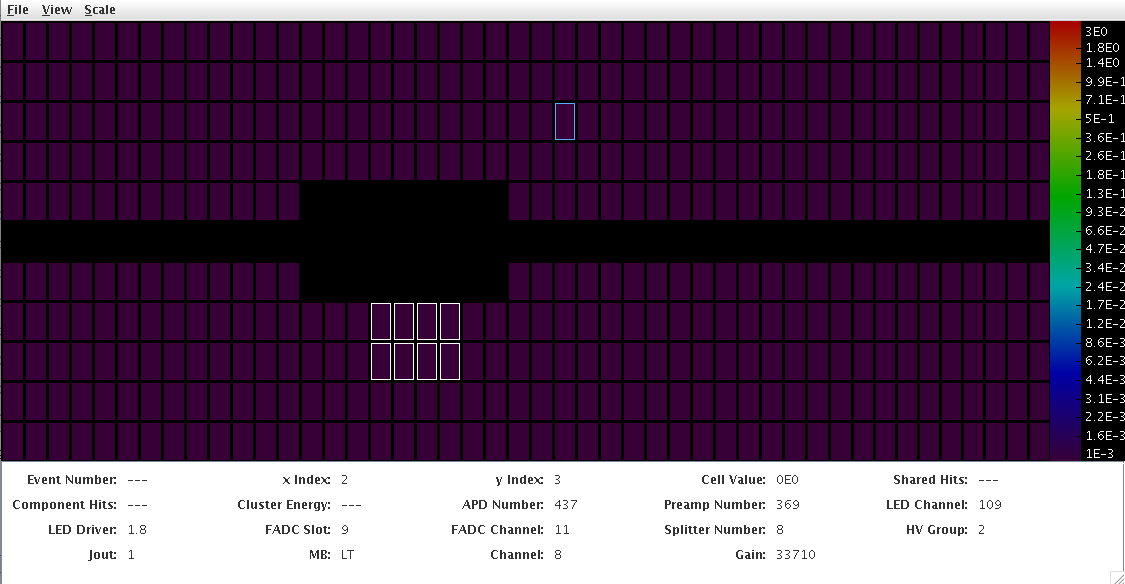
\includegraphics[width=16cm]{pics/kylesGui.png}
%\    \caption{The FT-Cal event display can be used to get channel mappings.  The blue-highlighted channel's mappings are shown in the table.  The white-highlighted channels correspond to the filtering applied via the {\bf View} menu, in this case HV group 25 on bottom.\label{fig:kylesGui}}
%\\end{figure}
%\%\%\%\%\%\%\%\%\%\%\%\%\%\%\%\%\%\%\%\%\%\%\%\%\%\%\%\


\section{Opening the Hodoscope}

This requires 2 people.  Extreme care must be taken for all fibres and cabling during this process.  

%The required tools are shown in Table ~\ref{tab:tools}.  The blue-handled chain-winches and metric crescent wrenches should be in the HPS cabinet on the pie tower.  The rest should be retrieved from the toolboxes on the Hall-B floor.  While one can get by with only half the number of wrenches of each type, it is fastest to have the full list. 
%
%\begin{table}[htbp]\centering
%    \begin{tabular}{c|l}\hline
%        Count & Type \\\hline
%4&   ECAL-ONLY chain winches (blue-handled)\\
%4&   15/16" crescent wrenches for rod bolts\\
%2&   11 mm crescent wrenches for lateral cossbar supports (over beampipe)\\
%2&   6 mm hex/allen wrenches for longitudinal crossbar supports (on far left/right)\\
%2&   3/16" hex/allen wrenches for support plates\\
%2&   medium-sized flathead screwdrivers\\\hline
%    \end{tabular}
%    \caption{Items used to open the calorimeter. \label{tab:tools}}
%\end{table}
%
%{\bf\em PLEASE return ALL tools back to where you found them.}

\section{Disconnection of a Channel and Preamplifier Replacement}
     
 In last resort, to recover a HV group that is tripping one can disconnect the faulty channel causing trouble. To do so, you need to find exactly which channel is involved! It might be obvious from data, if the channel was already very noisy, else you will have to test the channels of the group one by one. This is a lengthy operation and should only be attempted with the authorization of the run coordinator and in coordination with the FT-Cal Group. It necessitates that the Hall-B crew moves the FT-Cal out of the beam line and to open it.




\end{document}
